%% Author: Daniel Kaplan
%% Subject: 






Given data and a model design, the computer will find the model
function and model values for you.  
As an example, consider the Current Population
Survey  data \datasetCPS~.  Suppose you want to build a model with
\VN{wage} as a response variable and \variableName{age} and
\VN{sex} as explanatory variables incorporated as main
terms.  Also include the intercept term, as usual.

Using the model design language, this model is \model{\VN{wage}}{1 + \VN{age} + \VN{sex}}.

You first need to read in the data frame.  
\begin{Schunk}
\begin{Sinput}
 w = fetchData("cps.csv")
\end{Sinput}
\end{Schunk}


Next, use the \texttt{lm} operator to find the model function:
\begin{Schunk}
\begin{Sinput}
 mod1 = lm( wage ~ 1 + age + sex, data=w)
\end{Sinput}
\end{Schunk}


The two arguments are:
\begin{description}
\item[the model design] \model{\VN{wage}}{1 + \VN{age} + \VN{sex}}. 
\item[the data to be used]  This always looks like \texttt{data=w}
  where the name of the data frame is used.
\end{description}

The \texttt{mod1 = }... part of the command simply gives the model a
name so that you can use it later on.  If you construct more than one
model, it makes sense to give them different names.  But don't re-use
the name of the data frame; a name can be used for only one thing at a
time.

In making a graph of the function, the model values will always be
plotted on the vertical axis.  But you have a choice of what to put on
the horizontal axis.  Here are the commands which use the
\texttt{xyplot} operator:

\paragraph{Model values versus \VN{age}}.
  
\begin{Schunk}
\begin{Sinput}
 xyplot( fitted(mod1) ~ age, data=w )
\end{Sinput}
\end{Schunk}
  
\centerline{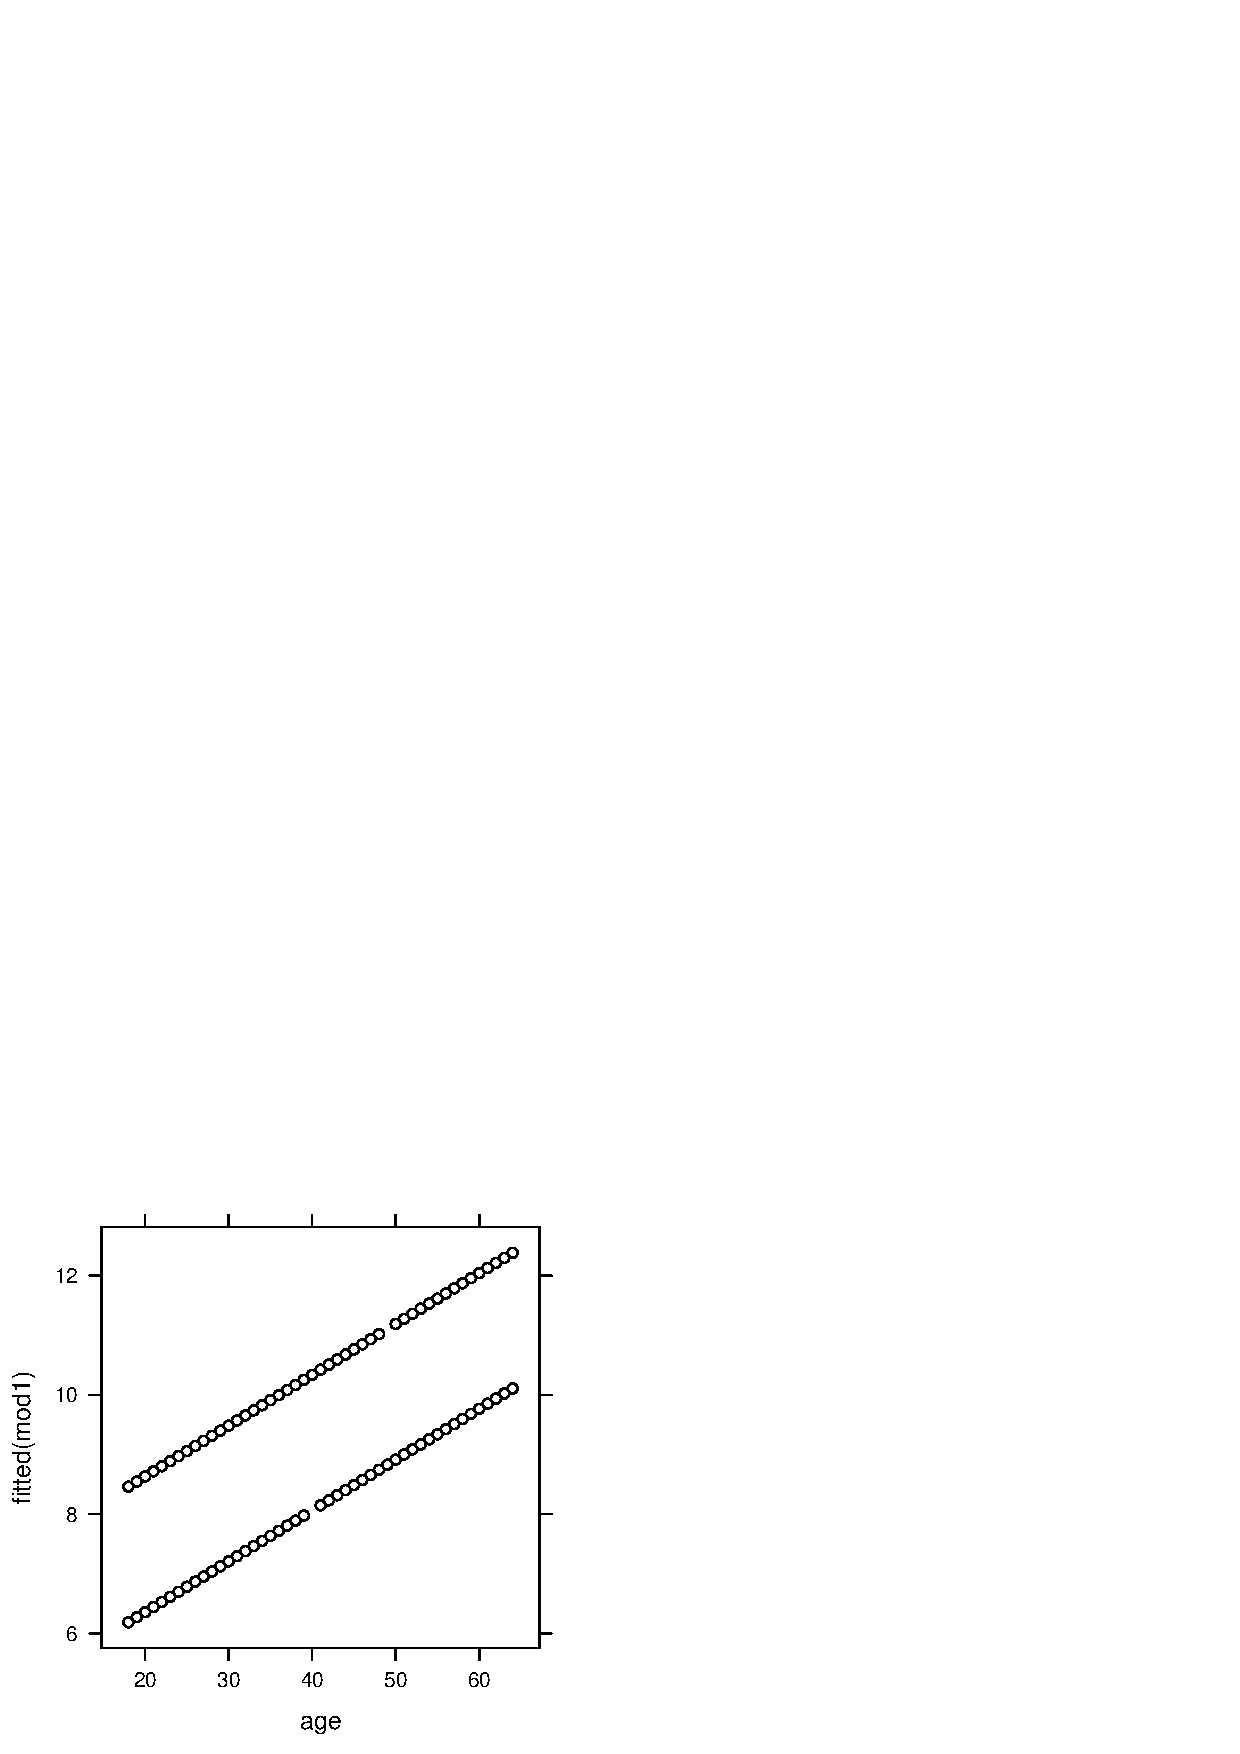
\includegraphics[width=2.5in]{Figures/fig-gmf1}}

\paragraph{Model values versus \VN{sex}}.

\begin{Schunk}
\begin{Sinput}
 print(xyplot( fitted(mod1) ~ sex, data=w ))
\end{Sinput}
\end{Schunk}
\centerline{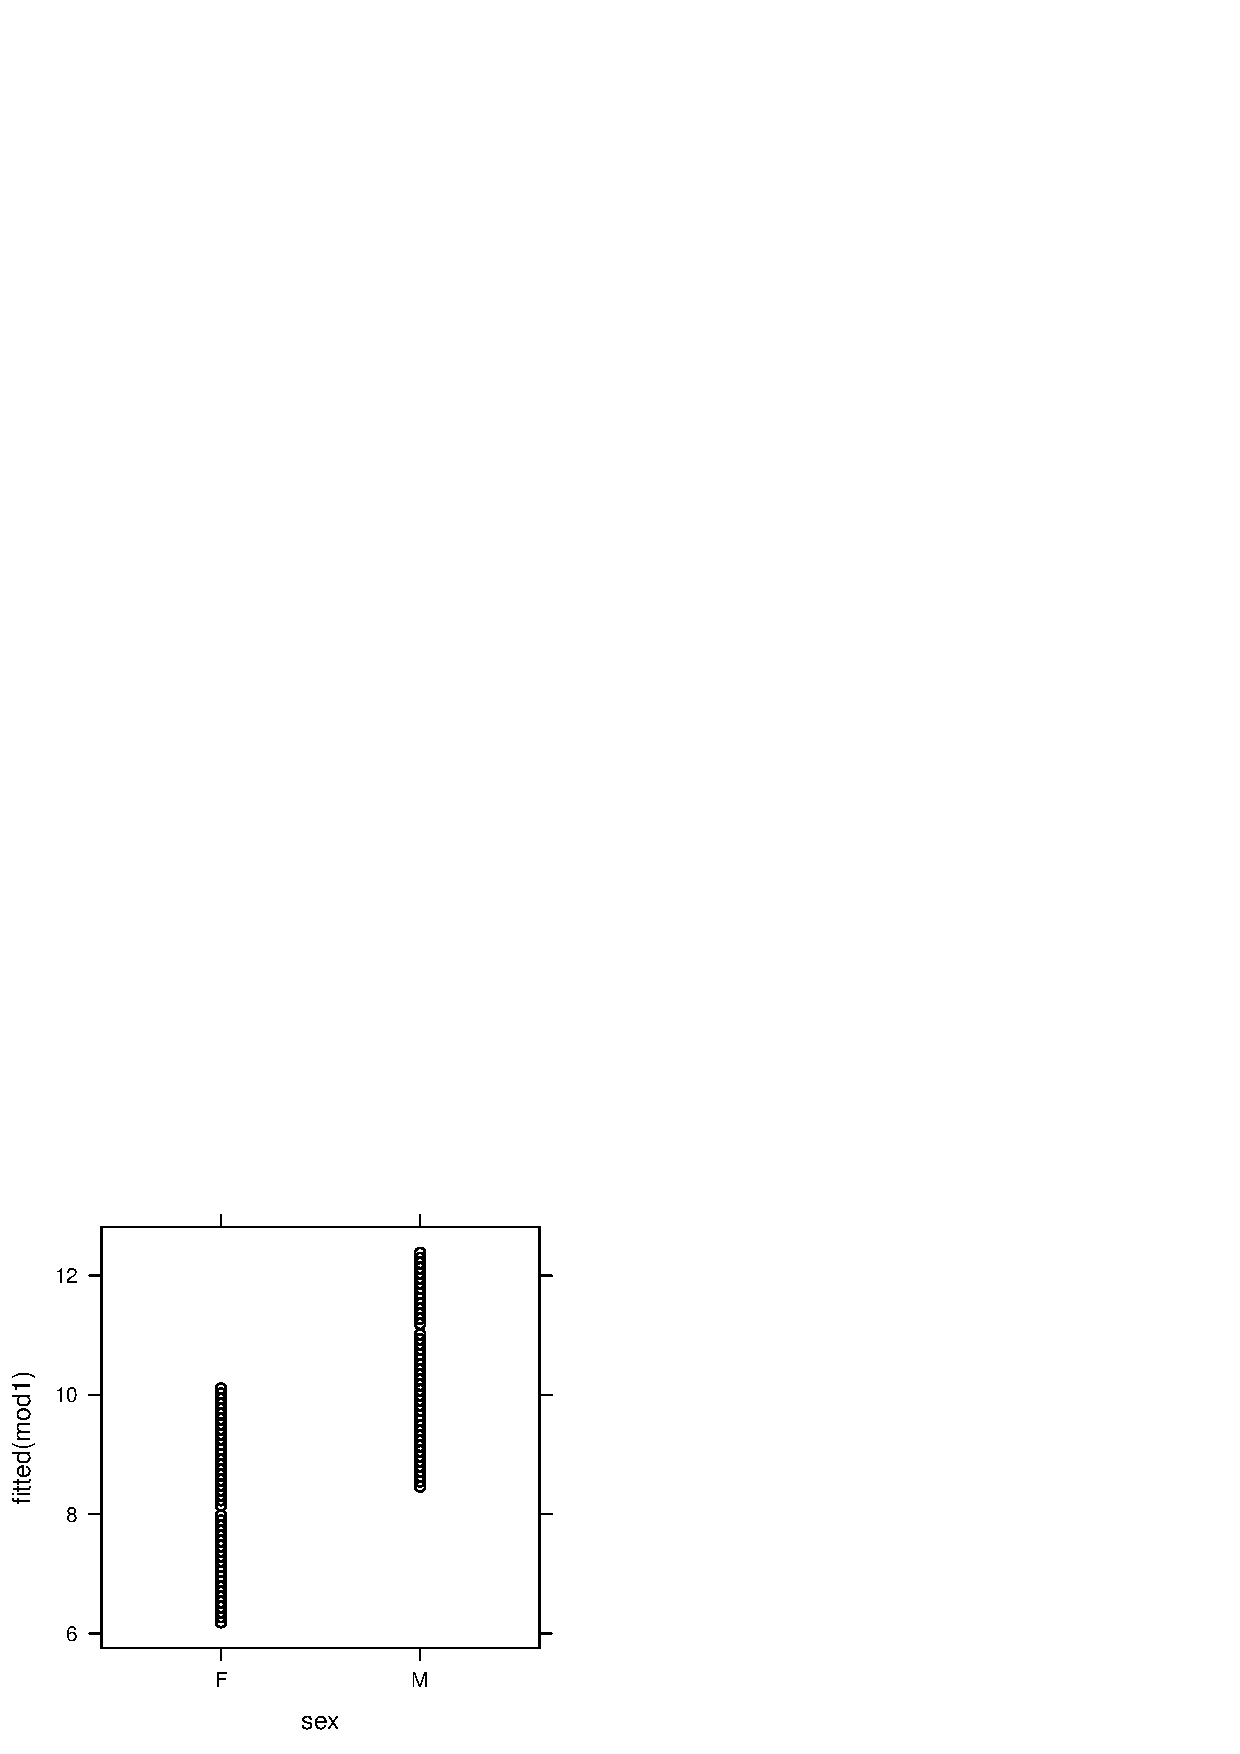
\includegraphics[width=2.5in]{Figures/fig-gmf2}}


The fitted model values can be accessed with \texttt{fitted(mod1)}.
The choice of which explanatory variable to plot on the horizontal
axis is specified by the name following the \verb.~. sign in the
plotting command.  Remember to include the name of the data frame in
the last argument: \texttt{data=w}.


Some elaborations are possible.

\paragraph{Show the response variable} in addition to the model values.
  This involves putting the response variable name to the left of the
  \verb.~. sign:

\begin{Schunk}
\begin{Sinput}
 print(xyplot( wage + fitted(mod1) ~ age, data=w ))
\end{Sinput}
\end{Schunk}

The \texttt{+} sign means ``plot both,'' not addition.

\centerline{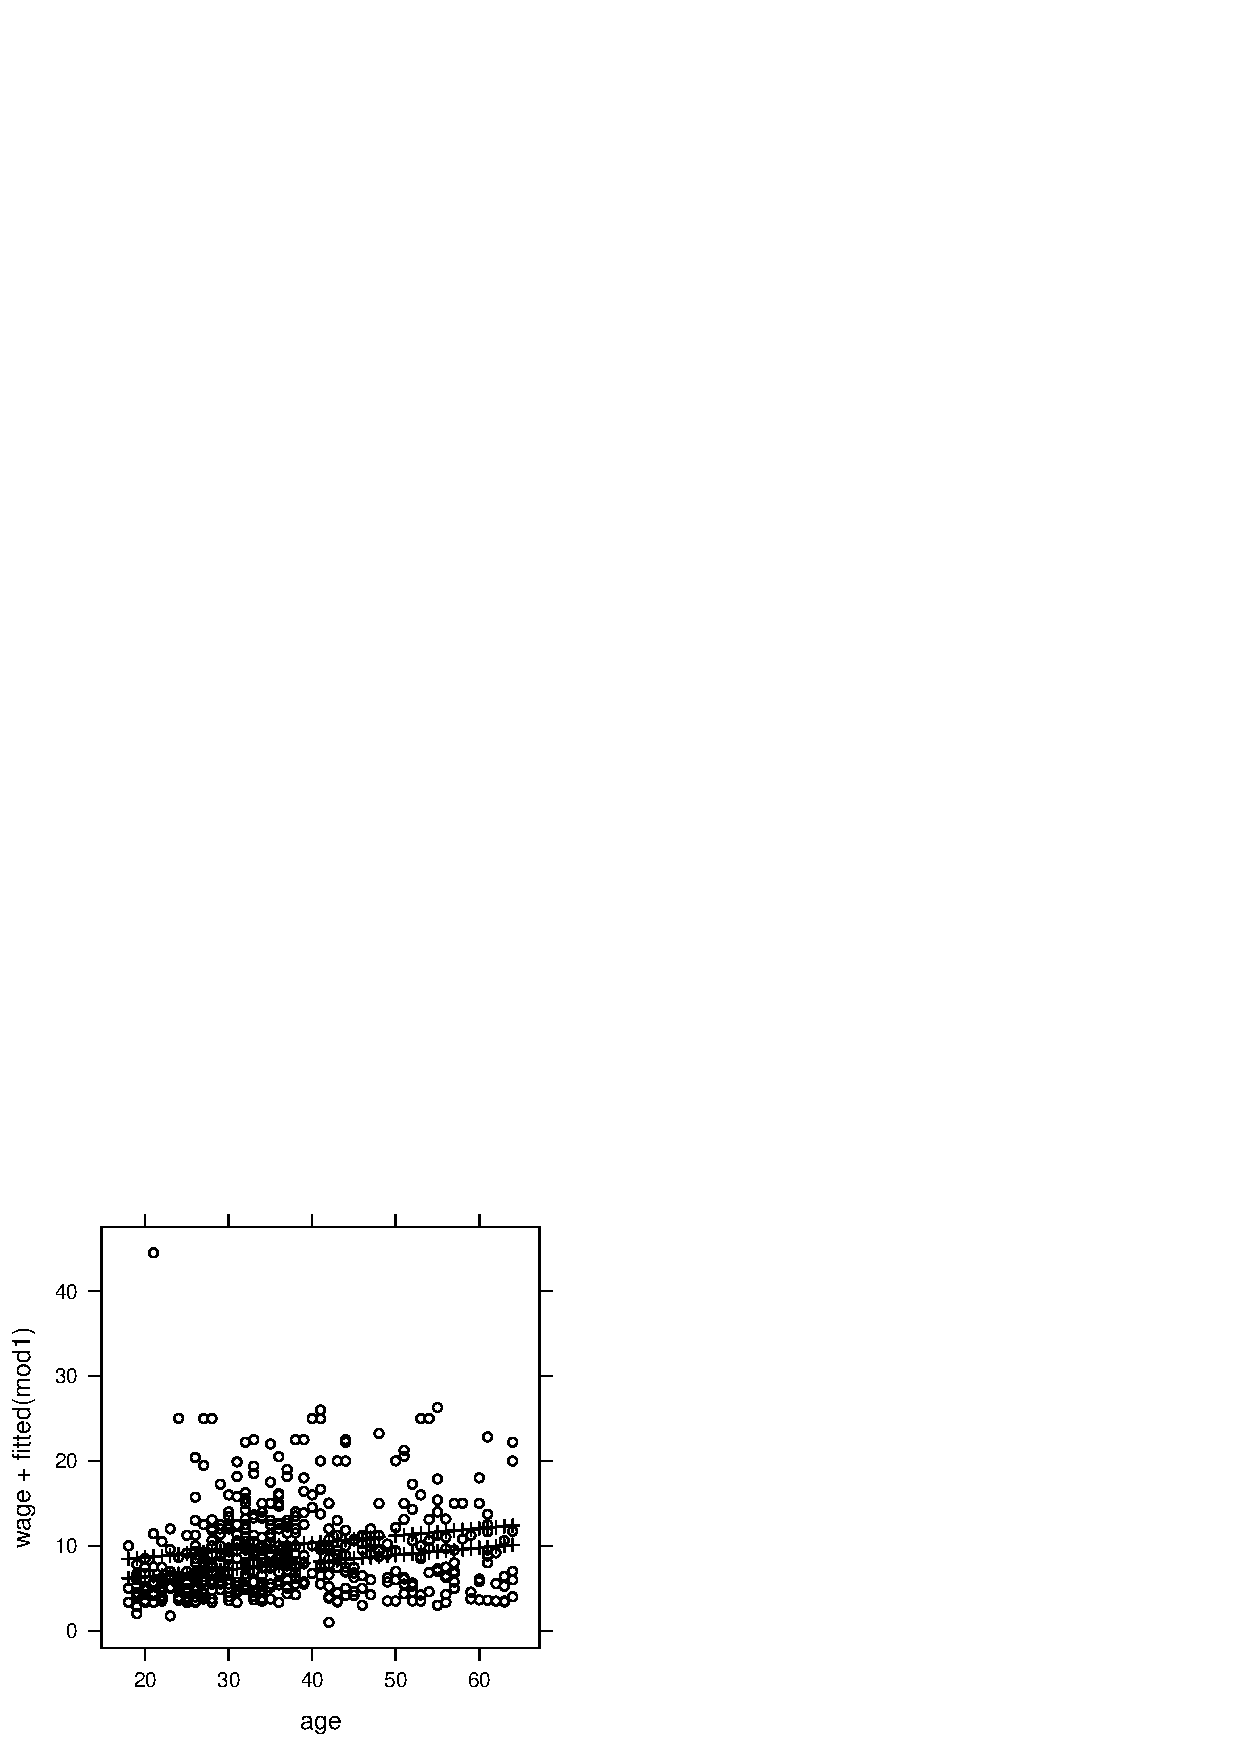
\includegraphics[width=2.5in]{Figures/fig-gmf3}}


\paragraph{Break up the display} according to one or more categorical
  variables.

\begin{Schunk}
\begin{Sinput}
 xyplot( wage + fitted(mod1) ~ age | sex, data=w )
\end{Sinput}
\end{Schunk}

This uses a vertical bar followed by the name of the categorical
variable.  Each of the levels of the variable to the right of the vertical bar
\verb+|+ will have a separate plot, so in the graphics it's females in
one plot and males in the other.

\centerline{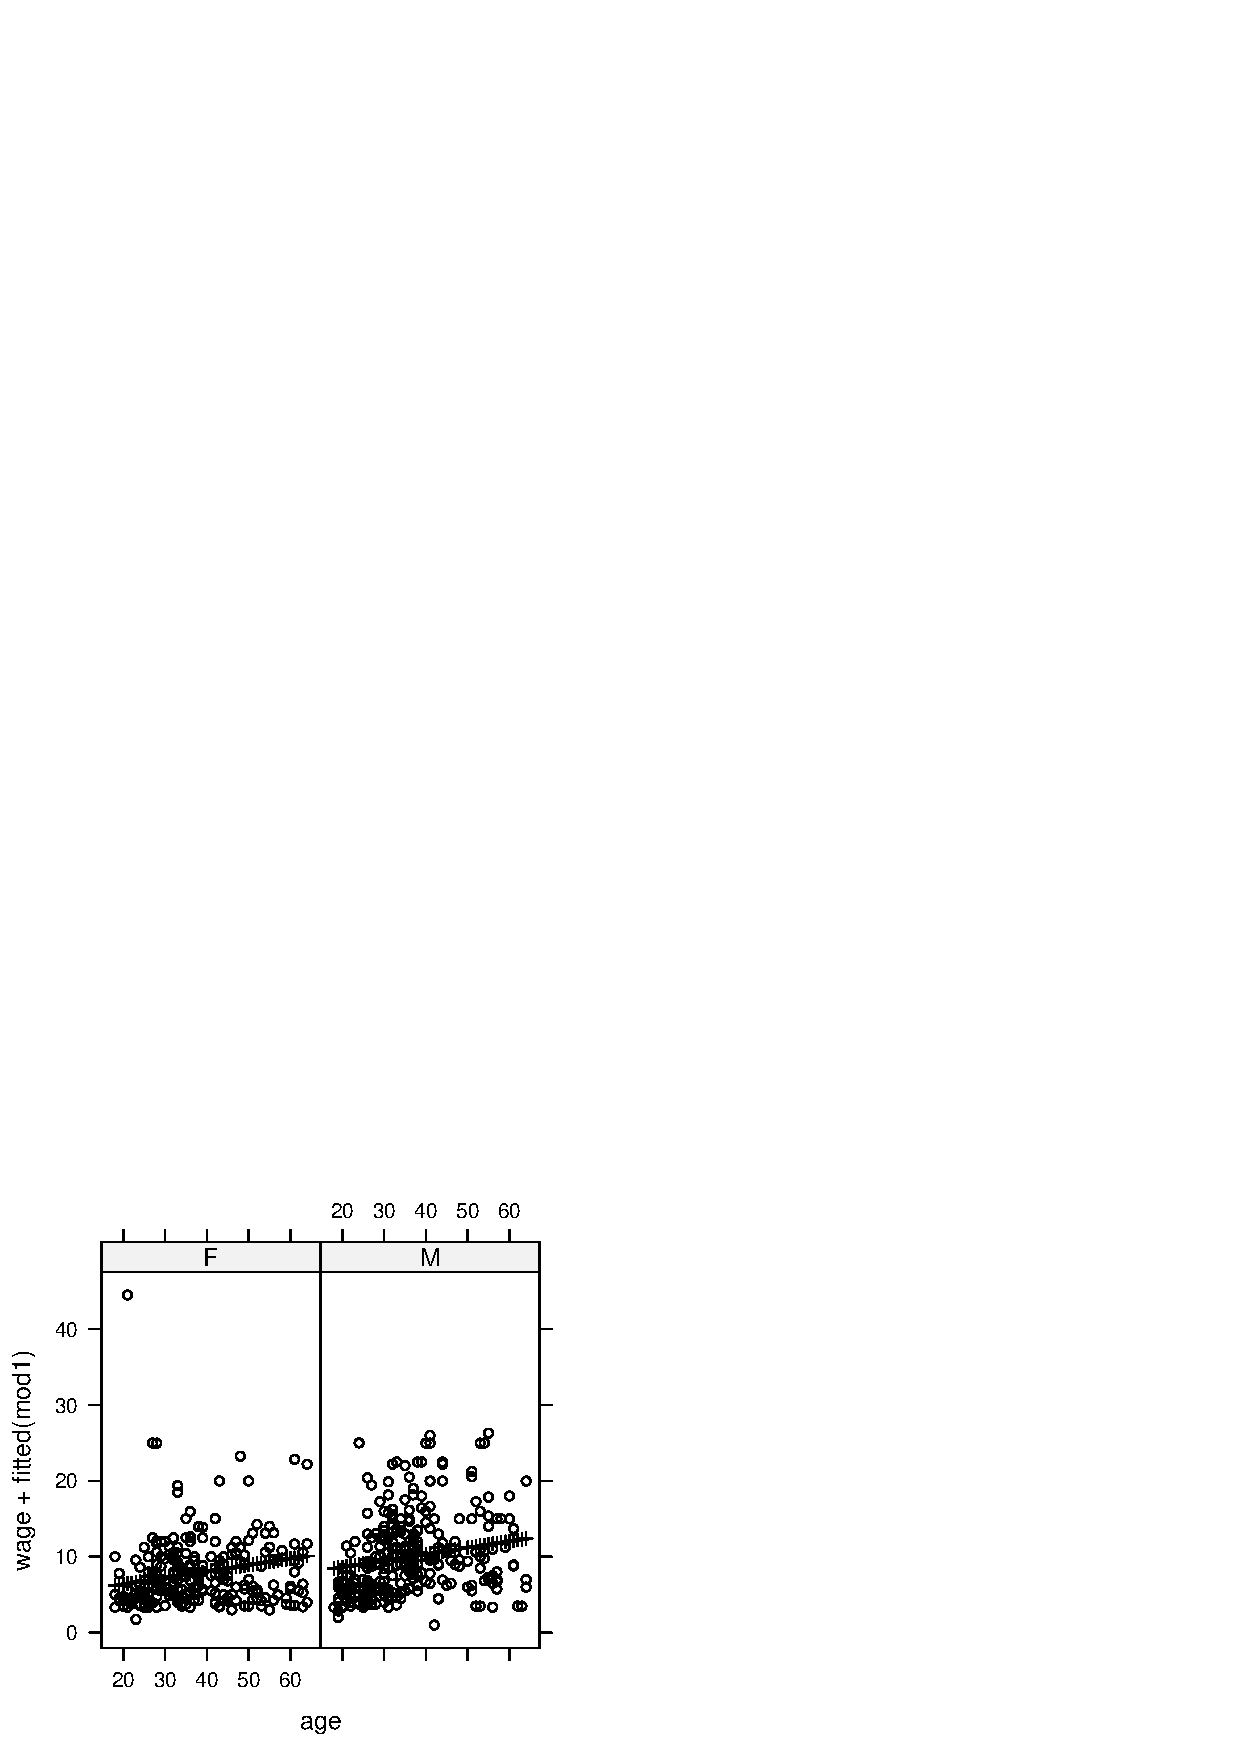
\includegraphics[width=2.5in]{Figures/fig-gmf4}}


A different way to break up the display makes it easier to compare the
model values for the different groups:

\begin{Schunk}
\begin{Sinput}
 xyplot(wage+fitted(mod1) ~ age,groups=sex,data=w)
\end{Sinput}
\end{Schunk}


\centerline{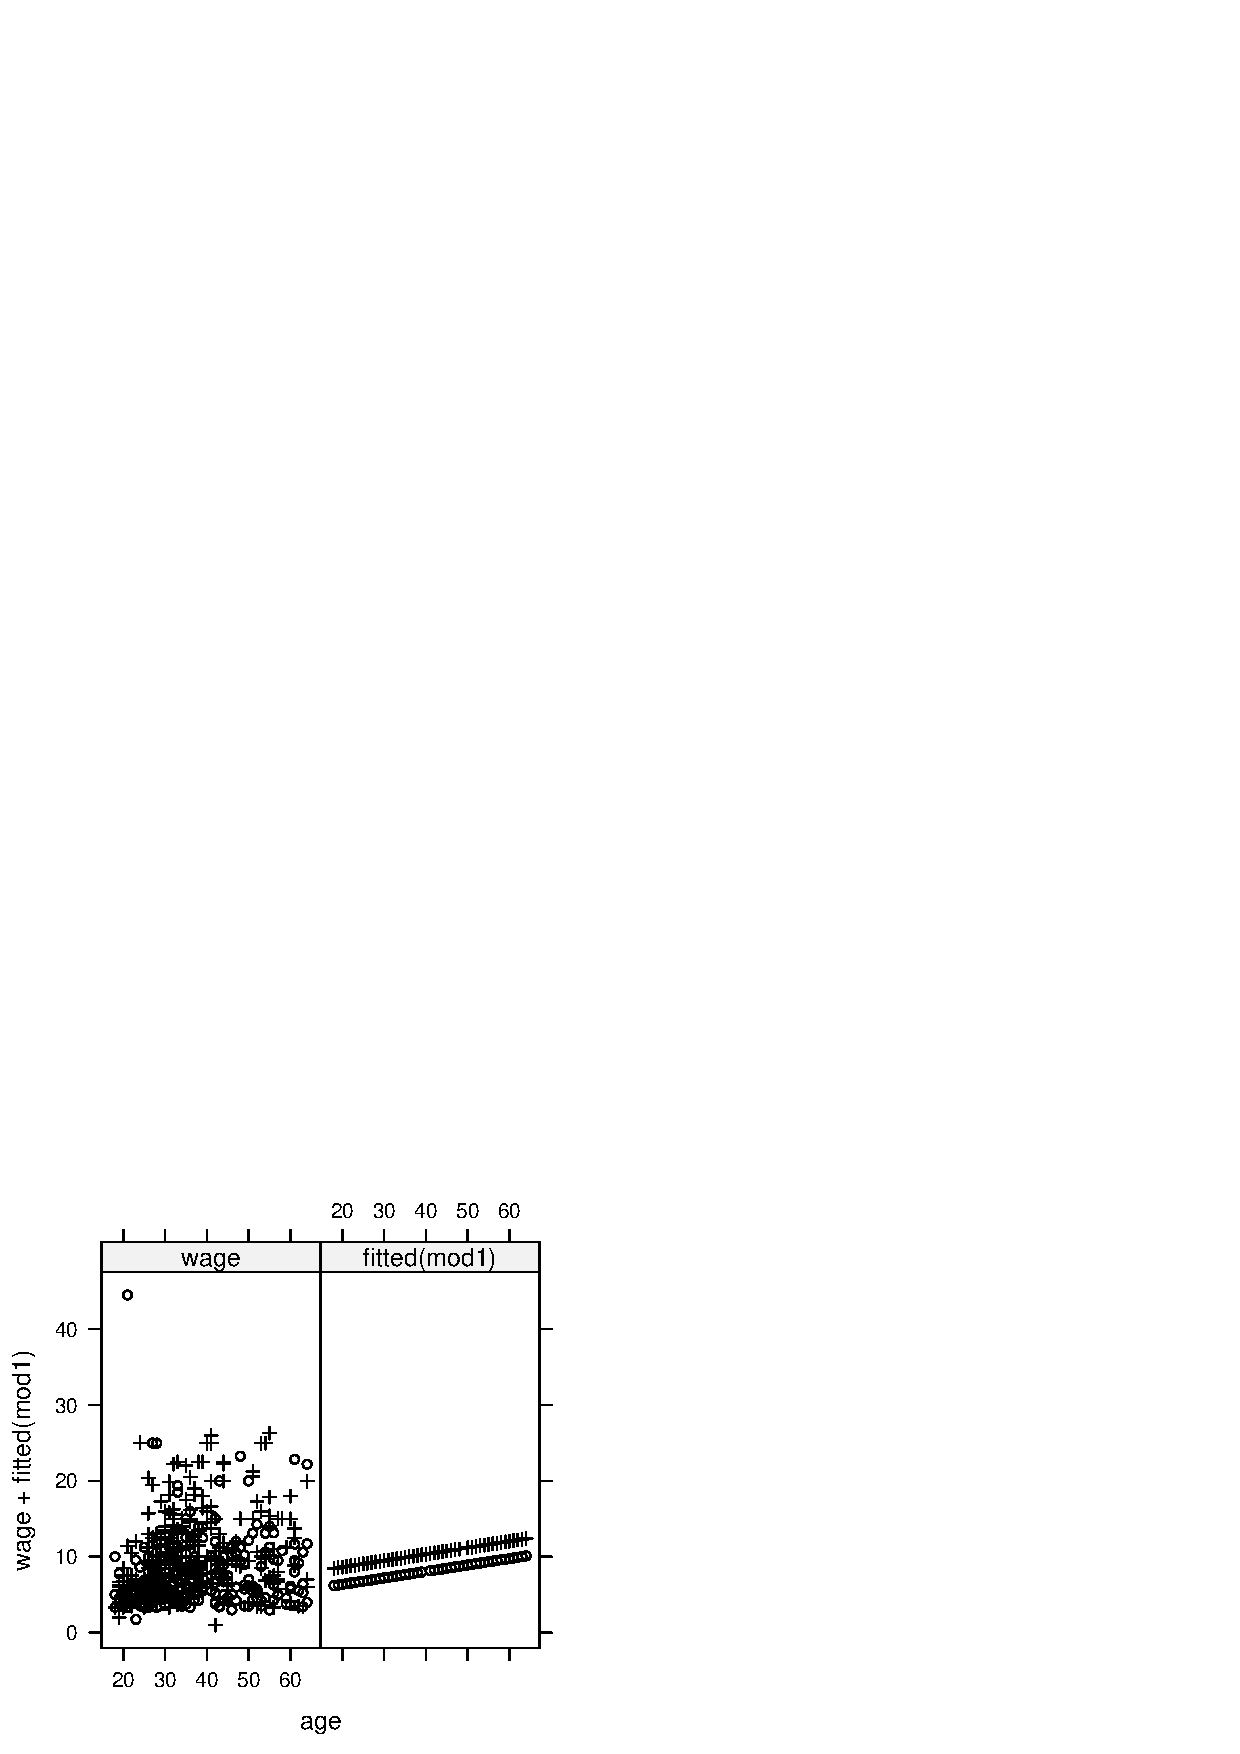
\includegraphics[width=2.5in]{Figures/fig-gmf5}}


